\documentclass[a4paper, 11pt]{report}
\usepackage{comment} % enables the use of multi-line comments (\ifx \fi) 
\usepackage{lipsum} %This package just generates Lorem Ipsum filler text. 
\usepackage{fullpage} % changes the margin
\usepackage[section]{placeins}
\usepackage[a4paper, total={7in, 10in}]{geometry}
\usepackage[fleqn]{amsmath}
\usepackage{amssymb,amsthm}  % assumes amsmath package installed
\newtheorem{theorem}{Theorem}
\newtheorem{corollary}{Corollary}
\usepackage{graphicx}
\usepackage{grffile}
\usepackage[maxfloats=256]{morefloats}
\maxdeadcycles=1000
\usepackage{tikz}
\usepackage{bm}
\usetikzlibrary{arrows}
\usepackage{verbatim}
\usepackage{listings}
%\usepackage[numbered]{mcode}
\usepackage{float}
\usepackage{tikz}
\usetikzlibrary{shapes,arrows}
\usetikzlibrary{arrows,calc,positioning}
\usetikzlibrary{arrows.meta}
\usepackage[
backend=biber,
style=ieee,
sorting=none
]{biblatex}
\addbibresource{bibliography.bib}

\tikzset{
	block/.style = {draw, rectangle,
		minimum height=1cm,
		minimum width=1.5cm},
	input/.style = {coordinate,node distance=1cm},
	output/.style = {coordinate,node distance=4cm},
	arrow/.style={draw, -latex,node distance=2cm},
	pinstyle/.style = {pin edge={latex-, black,node distance=2cm}},
	sum/.style = {draw, circle, node distance=1cm},
}
\usepackage{xcolor}
\usepackage{mdframed}
%\usepackage[shortlabels]{enumitem}
\usepackage{enumitem}
\usepackage{setspace} % for \onehalfspacing and \singlespacing macros
\onehalfspacing 
\usepackage{etoolbox}
\AtBeginEnvironment{quote}{\par\singlespacing\small}
%\usepackage{indentfirst}
\setlength{\parindent}{4em}
\setlength{\parskip}{1em}
\allowdisplaybreaks
\usepackage{hyperref}


\renewcommand{\thesubsection}{\thesection.\alph{subsection}}


\renewcommand{\qed}{\quad\qedsymbol}
%%%%%%%%%%%%%%%%%%%%%%%%%%%%%%%%%%%%%%%%%%%%%%%%%%%%%%%%%%%%%%%%%%%%%%%%%%%%%%%%%%%%%%%%%%%%%%%%%%%%%%%%%%%%%%%%%%%%%%%%%%%%%%%%%%%%%%%%

\title{Inferring trader information stream classification using chain graphs}
\author{Ted Watters}
\begin{document}
\maketitle


\begin{abstract}
	Create a synthetic data set from an agent-based model using NetLogo. Then, conduct chain graph analysis to see how accurately we can infer the number of trader classification categories, and what their probabilities are, given observed trading activity and information streams. As a possible extra, run a Monte Carlo simulation using the chain grain and then compare the original synthetic data set to the Markov Chain Monte Carlo results.
\end{abstract}\
\tableofcontents
\chapter{Introduction}
\section{The Market}
Consider the following agent-based market model, based on Cont's work~\cite{ghoulmie_cont_nadal_2005}. 

\begin{quote}
	Our model describes a market where a single asset, whose price is denoted by $p_{t}$ , is traded by
	$N$ agents. Trading takes place at discrete periods $t = 0, 1, 2,\dots$. We will see that, provided
	the parameters of the model are chosen in a certain range, we will be able to interpret these
	periods as "trading days". At each period, agents have the possibility of sending an order to
	the market for buying or selling a unit of asset: denoting by $\phi_{i}(t)$ the demand of the agent,
	we have $\phi_{i}(t) = 1$ for a buy order and $\phi_{i}(t) = -1$. We allow the value $\phi_{i}(t)$ to be zero; the
	agent is then inactive at period $t$. The inflow of public information is modeled by a sequence
	of IID Gaussian random variables $(\epsilon_{t},t = 0, 1, 2,\dots)$ with $t \sim N(0, D^{2})$.
\end{quote}
Diverging from this paper, in the model of this market, consider two independent public information streams $\epsilon_{main,t}$ and $\epsilon_{reddit,t}$, rather than a single information stream $\epsilon_{t}$.
\begin{quote}
	The signal $\epsilon_{t}$ [or in this case, $\epsilon_{main,t}$ and $\epsilon_{reddit,t}$] is a forecast of
	the future return $r_{t}$ and each agent has to decide whether the information conveyed by $\epsilon_{t}$ is
	significant, in which case she will place a buy or sell an order according to the sign of$\epsilon_{t}$.
\end{quote}
\textbf{Updated needed to this section related to how threshold $\theta(t)$ varies with time, relative to current return.}
\begin{quote}
	The trading rule of each agent $i = 1,..., N$ is represented by a \dots decision
	threshold [ $\theta_{i} \sim U(0,1)$]. The threshold [ $\theta_{i}$ ] can be viewed as the agent’s (subjective) view on volatility.
	The trading rule we study may be seen as a stylized example of threshold behaviour: without
	sufficient external stimulus [$(|\epsilon_{t}| \leq \theta_{i})$], an agent remains inactive $\phi_{i}(t) = 0$.
\end{quote}
In this case, since we have two information streams $\epsilon_{main,t}$ and $\epsilon_{reddit,t}$ we must define how an agent consumes them. Consider two classes of agents:
\begin{itemize}
	\item [$\rho_{i} = 0$] Consumes only main information stream
	\item [$\rho_{i} = 1$] Consumes both the main and reddit information streams, with a single set importance factor $\alpha \in [0,1]$ determining the relative weight of each information stream to the agent's decision making. 
\end{itemize}
The class of each agent does not vary with time, and is randomly determined, based on a single set reddit proportion factor $\beta \in [0,1]$. Thus:
\begin{equation}
\phi_{i}(t) = \begin{cases}
	1 & \rho_{i}=0,\epsilon_{main,t}>\theta_{i} \\
	1 & \rho_{i}=1,(\beta \epsilon_{reddit,t} + (1-\beta)\epsilon_{main,t}) > \theta_{i}\\
	0 & \rho_{i}=0, |\epsilon_{main,t}| \leq \theta_{i} \\
	0 & \rho_{i}=1, |\beta \epsilon_{reddit,t} + (1-\beta)\epsilon_{main,t}| \leq \theta_{i} \\
	-1 & \rho_{i}=0,\epsilon_{main,t}<\theta_{i} \\
	-1 & \rho_{i}=1,(\beta \epsilon_{reddit,t} + (1-\beta)\epsilon_{main,t}) < \theta_{i}\\
\end{cases}
\end{equation}
\begin{quote}
	The excess demand is then given by $Z_{t} = \sum_{i=1}^{N} \phi_{i}(t)$
\end{quote}
In this market, consider asset price at time $t$ defined by:
\begin{equation}
	p_{t} = p_{t-1} \exp \left( \frac{ Z_{t}}{\lambda N}\right)
\end{equation}
Where the sum of trader actions $Z_{t}$ is clearly calculated before $p_{t}$, and $\lambda > 0$ is the normalized market depth such that $g'(0) = \frac{1}{\lambda}$. 

Thus, the general procedure (after market initialization) at each step $t$ is:
\begin{enumerate}
	\item Each trader $i$ makes a buy/ no-action/ sell decision $\phi_{i}(t)$, which is a function of agent class $\rho_{i}$ and information stream $\epsilon_{main,t}$ (and possibly importance factor $\beta$ and $\epsilon_{reddit,t}$).
	\item Price is updated based on previous price $p_{t-1}$, sum of trader actions $Z_{t}$, and 
\end{enumerate}
\section{The Agent Based Model}
	Full code for the NetLogo~\cite{netlogo} (version 6.2.2) model is available at \url{https://github.com/tedwatters/info-stream/}. This repository is private for employer sensitivity reasons; however, please email \url{ted.watters@gmail.com} for access. Entire code file are included in the appendix \autoref{append:netlogo}, with snippets of interest in the main body of this report.
	
	The general procedure:
	\begin{lstlisting}
		to go
			set z 0
			set vol 0
			create-information
			ask traders [set done? false]
			while [count traders with [not done?] > 0]
			[ask traders [trade-2]]
			calculate-price
			calculate-return
			set vol sum [abs my-action] of traders
			;let t int (count traders * %-change)
			ask n-of (count traders * %-change) traders [change-threshold]
			if not write-output? [do-plots]
			;ask traders [move-around]
			if write-output? [do-output]
			tick
			if ticks > maxTicks [set write-output? false file-close-all stop]
		end
	\end{lstlisting}
	
	\noindent For the information streams, the main stream has information with a negative bias at ticks 495-500. Between 500-1,000, reddit information stream has a positive bias
	
	\begin{lstlisting}
	to create-information
		ifelse not newInfo?
		[
		ifelse paper?
		;; paper case
		[set current-info random-normal 0 (d ^ 2)
		]
		
		[set current-info random-normal 0 d] ;; original line
		]
		[
		;;set current-info current-info + first shuffle [1 -1 0]
		;;set current-info random-normal 0 (d ^ 2)
		
		ifelse ticks > 500 and ticks < 1000
		[
		set current-reddit random-normal 0.1 (d ^ 2) 
		;set current-info random-normal 0 (d ^ 2)
		]
		[
		set current-reddit random-normal 0 (d ^ 2)
		;set current-info random-normal 0 (d ^ 2)
		]
		
		ifelse ticks > 495 and ticks < 500
		[
		;set current-reddit random-normal 0.01 (d ^ 2)
		set current-info random-normal -0.01 (d ^ 2)
		]
		[
		;set current-reddit random-normal 0 (d ^ 2)
		set current-info random-normal 0 (d ^ 2)
		]
		
		;;set current-reddit current-reddit + first shuffle [1 1 1 1 1 -1 -1 -1 -1 0 0 0 0 0 0 0 0 0 0]
		]
	end
	\end{lstlisting}
	
	\noindent Trade decisions are made by:
	\begin{lstlisting}
	to trade-2
		;; for now only looking at paper case
		ifelse useBothFeeds? and myRedditUser
		[
		ifelse ((redditImportance * current-reddit) + ((1 - redditImportance) * current-info)) < (-1 * my-threshold) or ((redditImportance * current-reddit) + ((1 - redditImportance) * current-info)) > my-threshold
		[
		ifelse ((redditImportance * current-reddit) + ((1 - redditImportance) * current-info)) > 0
		[set my-action 1 set z z + 1][set my-action -1 set z z - 1]
		]
		[set my-action 0]
		]
		[
		;; paper case
		ifelse current-info < (-1 * my-threshold) or current-info > my-threshold
		[
		ifelse current-info > 0
		[set my-action 1 set z z + 1][set my-action -1 set z z - 1]
		]
		[set my-action 0]
		]
		set done? true
	end
	\end{lstlisting}
	
	And to calculate the updated price:
	\begin{lstlisting}
	to calculate-price
		set previous-price current-price
		;;set current-price sum [my-action] of traders
		set g ((z / (count traders)) / lamda)  ;; this is correct
		;; g is the price impact function which is a positive functin?
		;; ln ( p_t / p_{t-1 } ) = g -> e^g * p_{t-1} = p(t) ?
		set current-price exp g * previous-price
	end
	\end{lstlisting}
	
	This model produces a time series that includes:
	\begin{itemize}
		\item $phi_{i}(t)$, trader $i$ buy/ no-action/ sell
		\item $\sum_{i=1}^{N} | \phi_{i}(t) |$, the volume of traders wanting to trade
		\item $Z_{t}$, excess demand
		\item $p_{t}$, price
		\item $\epsilon_{main,t}$ and $\epsilon_{reddit,t}$, the info streams
	\end{itemize}

	For example, see ~\autoref{ex_price}, ~\autoref{ex_vol}, and ~\autoref{ex_info}.
\begin{figure}[h!]
	\caption{Current Price}
	\label{ex_price}
	\includegraphics[width=\textwidth]{../plots/priceRR0-RI0.1.png}
\end{figure}

\begin{figure}[h!]
	\caption{Volume}
	\label{ex_vol}
	\includegraphics[width=\textwidth]{../plots/volRR0-RI0.1.png}
\end{figure}

\begin{figure}[h!]
	\caption{Info Streams}
	\label{ex_info}
	\includegraphics[width=\textwidth]{../plots/infoRR0-RI0.1.png}
\end{figure}

\chapter{Bayesian Inference}	
\section{The Template Model}
This agent based model can be represented by a template chain graph shown in ~\autoref{chain_graph}. \textbf{Need to update representation of $\theta_{i}(t)$}. In this case, there are two main template groups. The first contains node specific to an agent $i$, and the second refers to nodes specific to time $t$. The gray nodes represent latent variables that we cannot observe, whereas the transparent nodes are ones we can observe. 

\begin{figure}[h]
	\centering
	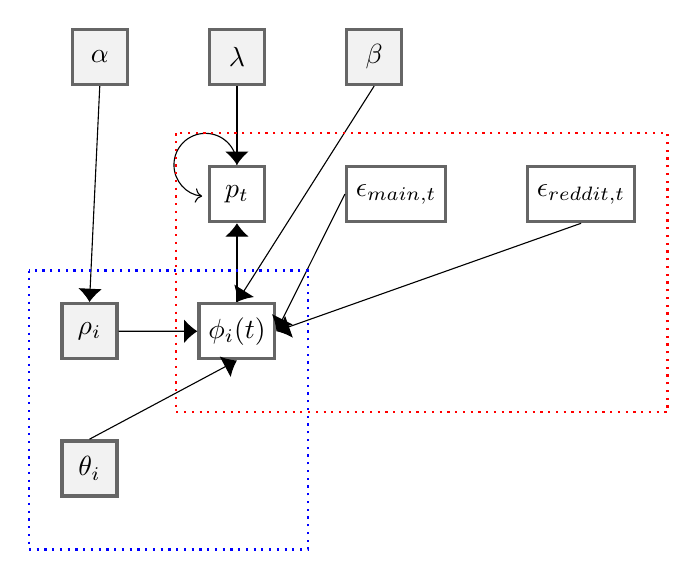
\begin{tikzpicture}[
	squarednode/.style={rectangle, draw=black!60, fill=black!5, very thick, minimum size=7mm},
	resultnode/.style={rectangle, draw=black!60, very thick, minimum size=7mm},	
	scale = 0.2
	]
	%Nodes
	\node[squarednode, align=center]      (lambda)                              {$\lambda$};	
	\node[squarednode, align=center]      (importance)     [right=of lambda]                        {$\beta$};
	\node[squarednode, align=center]      (proportion)     [left=of lambda]                          {$\alpha$};		
	\node[resultnode, align=center]        (price)       [below=of lambda] {$p_{t}$};		
	\node[resultnode, align=center]        (action)       [below =of price] {$\phi_{i}(t)$};				
	\node[squarednode, align=center]        (class)       [left=of action] {$\rho_{i}$};
	\node[resultnode, align=center]        (main)       [right=of price] {$\epsilon_{main,t}$};				
	\node[resultnode, align=center]        (reddit)       [right=of main] {$\epsilon_{reddit,t}$};
	\node[squarednode, align=center]      (threshold)     [below=of class]      {$\theta_{i}$};					
%	%Lines
	\draw[-{Latex[width=3mm]}] (importance.south) -- (action.north);
	\draw[-{Latex[width=3mm]}] (proportion.south) -- (class.north) ;
	\draw[-{Latex[width=3mm]}] (class.east) -- (action.west);
	\draw[-{Latex[width=3mm]}] (main.west) -- (action.east);
	\draw[-{Latex[width=3mm]}] (reddit.south) -- (action.east);
	\draw[-{Latex[width=3mm]}] (lambda.south) -- (price.north);
	\draw[-{Latex[width=3mm]}] (threshold.north) -- (action.south);
	\draw[-{Latex[width=3mm]}] (action.north) -- (price.south);
	\draw [->] (price.90) arc (0:264:20mm);
%	%rectangle
	\draw[red,thick,dotted] ($(price.north west)+(-2,2)$)  rectangle ($(reddit.south east)+(2,-12)$);
	\draw[blue,thick,dotted] ($(class.north west)+(-2,2)$)  rectangle ($(action.south east)+(2,-12)$);

	\end{tikzpicture}\\
	\caption{Template Chain Graph}
	\label{chain_graph}
\end{figure}

Our primary objectives are to accurately estimate $\alpha \in [0,1]$, $\lambda >0$, and $\beta \in [0,1]$ only given $p_{t}$, $\epsilon_{main,t}$, $\epsilon_{reddit,t}$, and $\phi_{i}(t)$.

\section{Inference Approach}

After transforming the data generated from the agent based model into a format that can be used for this analysis (code available in ~\autoref{append:r}), a graph representation can be created. One of the struggles here is that for the causact package, it does Bayesian inference using the greta package, which in turn uses a Hamilton Monte Carlo algorithm. Unfortunately, it cannot directly do inference on discrete random variables, which we would like to do for $\rho_{i}$. Since the parameter we really care about is $\alpha$, we can adjust $\rho_{i}$ and the decision making equation in $\phi_{i}(t)$ to work with a modified continuous $\rho_{i}$. In this case, the $\alpha$ that we are looking at ranges from $[0,0.5]$, so when interpreting the model's parameter estimates we need to multiply by a factor of 2 to get the actual $\alpha$
\begin{lstlisting}[language=R]
  # make the graph
	graph = dag_create() %>%
		dag_node("Decision","phi_o",
			rhs = uniform(-1,1),
			# rhs = uniform(phi[tp,ip]-0.1,phi[tp,ip]+0.1),
			data = trader_tick_phi,
			keepAsDF = TRUE
			) %>%
		dag_node("Trader Decision","phi",
			rhs = decision_function(rho[ip],betar,epsilon_reddit[tp],epsilon_main[tp],theta[ip]),
			# rhs = uniform(-1,1),
			# data = trader_decisions$value,
			dec = TRUE,
			child = "phi_o") %>%
		dag_node(descr = "Trader Classification",label = "rho",
			rhs = alpha+z,
			child = "phi") %>%
			dag_node(descr = "Proportion of Reddit Traders",label = "alpha",
			rhs = uniform(0,0.5),
			child = "rho") %>%
		dag_node(descr = "Trader Threshold", label = "theta",
			rhs = beta(2,2),
			child = "phi") %>%
			dag_node(descr =  "Reddit Importance Factor",label = "betar",
			rhs = uniform(0,1),
			child = "phi") %>%
		dag_node("Info Main","epsilon_main",
			data = trader_decisions$current.info,
			child = "phi") %>%
		dag_node("Info Reddit","epsilon_reddit",
			data = trader_decisions$current.reddit,
			child = "phi") %>%
		dag_node("Tick","t",
			data = trader_decisions$ticks,
			child="phi") %>%
		dag_node("Trader","i",
			data = as.numeric(trader_decisions$variable),
			child="phi") %>%
		dag_node("Rho_cut","z",
			rhs = uniform(0,0.5),
			child="rho") %>%
		dag_plate("Trader","ip",
			nodeLabels = c("rho","theta","i","phi","phi_o","z"),
			data = trader_decisions$variable) %>%
		dag_plate("Tick Plate","tp",
			nodeLabels = c("epsilon_reddit","epsilon_main","t","phi","phi_o"),
			data = trader_decisions$tick)
\end{lstlisting}
This code generates the following graphical representation ~\autoref{ex_graph}.
\begin{figure}[h!]
	\caption{Plate Graph}
	\label{ex_graph}
	\includegraphics[width=\textwidth]{../plots/graphRR0-RI0.1.png}
\end{figure}

Dark green nodes are observed, and the square node is a decision node


Running the inference itself is straightforward.

\begin{lstlisting}[language=R]
 	 gretaCode = graph %>% dag_greta(mcmc=FALSE)
	drawsDF = graph %>% dag_greta()
\end{lstlisting}

The greta code line generates the following code, which could be run separately as desired, but gives more insight into the model itself

\begin{lstlisting}[language=R]
## The below greta code will return a posterior distribution 
## for the given DAG. Either copy and paste this code to use greta
## directly, evaluate the output object using 'eval', or 
## or (preferably) use dag_greta(mcmc=TRUE) to return a data frame of
## the posterior distribution: 
epsilon_main <- as_data(trader_decisions$current.info)       #DATA
epsilon_reddit <- as_data(trader_decisions$current.reddit)   #DATA
t <- as_data(trader_decisions$ticks)                         #DATA
i <- as_data(as.numeric(trader_decisions$variable))          #DATA
phi_o <- as_data(trader_tick_phi)                            #DATA
ip     <- as.factor(trader_decisions$variable)   #DIM
tp     <- as.factor(trader_decisions$tick)   #DIM
ip_dim <- length(unique(ip))   #DIM
tp_dim <- length(unique(tp))   #DIM
alpha  <- uniform(min = 0, max = 0.5)                  #PRIOR
theta  <- beta(shape1 = 2, shape2 = 2, dim = ip_dim)   #PRIOR
betar  <- uniform(min = 0, max = 1)                    #PRIOR
z      <- uniform(min = 0, max = 0.5, dim = ip_dim)    #PRIOR
rho    <- alpha + z                                                                                                            #OPERATION
phi    <- decision_function(rho = rho[ip], betar = betar, er = epsilon_reddit[tp], em = epsilon_main[tp], theta = theta[ip])   #OPERATION
distribution(phi_o) <- uniform(min = -1, max = 1, dim = c(ip_dim,tp_dim))   #LIKELIHOOD
gretaModel  <- model(alpha,theta,betar,z)   #MODEL
meaningfulLabels(graph)
draws       <- mcmc(gretaModel)              #POSTERIOR
drawsDF     <- replaceLabels(draws) %>% as.matrix() %>%
dplyr::as_tibble()           #POSTERIOR
tidyDrawsDF <- drawsDF %>% addPriorGroups()  #POSTERIOR
\end{lstlisting}

This code then outputs confidence intervals for each parameter ~\autoref{ex_paramEst}. Of interest are the "alpha" and "betar" parameters.

\begin{figure}[h!]
	\caption{Parameter Estimate}
	\label{ex_paramEst}
	\includegraphics[width=\textwidth]{../plots/paramEstRR0-RI0.1.png}
\end{figure}

In the appendix, I've included data from multiple runs. In particular, we can notice that with the particular parameters set, only larger $\beta$ and $\alpha$ values generate large differences in pricing away from the baseline. This in turn makes the parameter estimates relatively similar across data runs, and makes the confidence for estimating $\alpha$ and $\beta$ lower. 

\chapter{Progress Planned}



\noindent Progress planned:
\section{Steps}
\begin{itemize}
\item Quality check inference
\item Create Monte Carlo generated time series from graph, and compare to original time series (bulk properties, such as mean, variance, autocorrelation, etc.)
\item Clean up report section, including adding mathematical detail about how I transformed $\rho_{i}$ to be continuous and why I needed to.
\end{itemize}
\section{Supporting Research}
This project is inspired by Cont's market model~\cite{ghoulmie_cont_nadal_2005}. From the abstract:
\begin{quote} 
	We propose an agent-based model of a single-asset financial market, described in terms of a small number of parameters, which generates price returns with statistical properties similar to the stylized facts observed in financial time series... The parsimonious structure of the model allows the identification of feedback and heterogeneity as the key mechanisms leading to these effects. 
\end{quote}
Next, it has been shown in Epstein~\cite{epstein2007generative} \textit{Chapter 8: The Emergence of Class in a Multi-Agent Bargaining Model} that:
\begin{quote}
	...We have argued that various kinds of social orders— including segregated, discriminatory, and class systems— can also arise through the decentralized interactions of many agents in which accidents of history become reinforced over time. In these path-dependent dynamics, society may self-organize around distinctions that are quite arbitrary from an a priori standpoint. Above, initially meaningless “tags” acquire socially organizing salience: tag-based classes emerge.
\end{quote}
	So in a bargaining model, similar to the financial market, classes can arise from small changes to initial conditions. In this project, I'm seeking to change information stream sources for individual traders, and then see if classification of traders emerge. 
	
	The main purpose of this project is to see how we can use probabilistic graphical models to infer this class structure from trading activity. We expect this structure to be at least partially directed, and there are some variables that are impossible to measure (without having the underlying model I'm using to create the synthetic data set). 
	
	Our class text ~\cite{koller2009} also reviews learning causal models with latent variables in 21.7. While we haven't gotten there in the class, this section alludes to 3 chapters in the text which deal with learning the structure of Bayesian networks. I'll review those. Additionally, I signed up to audit the Coursera ~\cite{coursera} class, which has lectures that I can watch sooner than what's available on blackboard
	
	Another research area includes latent conditional random fields. Example articles include Sun's 2013 work~\cite{sun2013}:
	\begin{quote}
		 We propose a perceptron-style method, latent structured perceptron, for fast discriminative learning of structured classification with hidden information. We also give theoretical analysis and demonstrate good convergence properties of the proposed method. Our method extends the perceptron algorithm for the learning task with hidden information, which can be hardly captured by traditional models. It relies on Viterbi decoding over latent variables, combined with simple additive updates.
	\end{quote}

	The trading data generated by the agent based model will be sequential, so understanding how that relates to the conditional random field is important Examples include this work ~\cite{sun2022}
	\begin{quote}
		...we propose a new multiview discriminant model based on conditional random fields (CRFs) to model multiview sequential data, called multiview CRF. It inherits the advantages of CRFs that build a relationship between items in each sequence. Moreover, by introducing specific features designed on the CRFs for multiview data, the multiview CRF not only considers the relationship among different views but also captures the correlation between the features from the same view. Particularly, some features can be reused or divided into different views to build an appropriate size of feature space. This helps to avoid underfitting problems caused by too small feature space or overfitting problems caused by too large feature space. In order to handle large-scale data, we use the stochastic gradient method to speed up our model.
	\end{quote}

	And this work ~\cite{abramson2016}
	
	\begin{quote}
		The claim of this paper is that CRF models
		also provide discriminative models to distinguish between types
		of sequence regardless of the accuracy of the labels obtained if
		we calibrate the class membership estimate of the sequence. We
		introduce and compare different neural network based linear-
		chain CRFs and we present experiments on two complex sequence
		classification and structured prediction tasks to support this
		claim.
	\end{quote}

	And this work ~\cite{lafferty2001}
	
	\begin{quote}
		We present conditional random fields, a framework for building probabilistic models to segment and label
		sequence data. Conditional random fields offer several advantages over hidden Markov models and
		stochastic grammars for such tasks, including the ability to relax strong independence assumptions
		made in those models. Conditional random fields also avoid a fundamental limitation of maximum
		entropy Markov models (MEMMs) and other discriminative Markov models based on directed graphical
		models, which can be biased towards states with few successor states. We present iterative parameter
		estimation algorithms for conditional random fields and compare the performance of the resulting
		models to HMMs and MEMMs on synthetic and natural-language data.
	\end{quote}

	And possibly this work ~\cite{thai2018}:
	
	\begin{quote}
		 Our model goes beyond the linear chain CRF to incorporate multiple hidden states per output label, but parametrizes their transitions parsimoniously with low-rank log-potential scoring matrices, effectively learning an embedding space for hidden states. This augmented latent space of inference variables complements the rich feature representation of the RNN, and allows exact global inference obeying complex, learned non-local output constraints. We experiment with several datasets and show that the model outperforms baseline CRF+RNN models when global output constraints are necessary at inference-time, and explore the interpretable latent structure. 
	\end{quote}

	And possibly this work ~\cite{neogi2019}:
	
	\begin{quote}
		Conditional Random Fields (CRF) are frequently applied for labeling and segmenting sequence data. Morency et al. (2007) introduced hidden state variables in a labeled CRF structure in order to model the latent dynamics within class labels, thus improving the labeling performance. Such a model is known as Latent-Dynamic CRF (LDCRF). We present Factored LDCRF (FLDCRF), a structure that allows multiple latent dynamics of the class labels to interact with each other. Including such latent-dynamic interactions leads to improved labeling performance on single-label and multi-label sequence modeling tasks. We apply our FLDCRF models on two single-label (one nested cross-validation) and one multi-label sequence tagging (nested cross-validation) experiments across two different datasets - UCI gesture phase data and UCI opportunity data.
	\end{quote}

	Once I've gained a good understanding of different methodologies, I also need to make sure there are some existing software packages which I can leverage. Examples include R's crf ~\cite{ling2019}, bnlearn ~\cite{scutari2021}, rstan ~\cite{guo2021}, BiDAG ~\cite{suter2021}, and BDgraph ~\cite{mohammadi2021}.

\chapter*{Bibliography}
\printbibliography

\chapter{Appendix}
\section{Graph}
%"for f in ./plots/*.png; do echo $( printf "\\\begin{figure}[h] \n\\caption{File: .$f} \n \\includegraphics[width=\\\textwidth]{.$f} \n \\\end{figure} \n"); done;"

\begin{figure}[h] \caption{File: ../plots/graphRR0-RI0.1.png} \includegraphics[width=\textwidth]{../plots/graphRR0-RI0.1.png} \end{figure}
\section{Info Stream}
\begin{figure}[h] \caption{File: ../plots/infoRR0-RI0.1.png} \includegraphics[width=\textwidth]{../plots/infoRR0-RI0.1.png} \end{figure}
\section{Parameter Estimates}
\begin{figure}[h] \caption{File: ../plots/paramEstRR0.05-RI0.1.png} \includegraphics[width=\textwidth]{../plots/paramEstRR0.05-RI0.1.png} \end{figure}
\begin{figure}[h] \caption{File: ../plots/paramEstRR0.05-RI0.3.png} \includegraphics[width=\textwidth]{../plots/paramEstRR0.05-RI0.3.png} \end{figure}
\begin{figure}[h] \caption{File: ../plots/paramEstRR0.05-RI0.5.png} \includegraphics[width=\textwidth]{../plots/paramEstRR0.05-RI0.5.png} \end{figure}
\begin{figure}[h] \caption{File: ../plots/paramEstRR0.05-RI0.7.png} \includegraphics[width=\textwidth]{../plots/paramEstRR0.05-RI0.7.png} \end{figure}
\begin{figure}[h] \caption{File: ../plots/paramEstRR0.05-RI0.png} \includegraphics[width=\textwidth]{../plots/paramEstRR0.05-RI0.png} \end{figure}
\begin{figure}[h] \caption{File: ../plots/paramEstRR0.1-RI0.1.png} \includegraphics[width=\textwidth]{../plots/paramEstRR0.1-RI0.1.png} \end{figure}
\begin{figure}[h] \caption{File: ../plots/paramEstRR0.1-RI0.3.png} \includegraphics[width=\textwidth]{../plots/paramEstRR0.1-RI0.3.png} \end{figure}
\begin{figure}[h] \caption{File: ../plots/paramEstRR0.1-RI0.5.png} \includegraphics[width=\textwidth]{../plots/paramEstRR0.1-RI0.5.png} \end{figure}
\begin{figure}[h] \caption{File: ../plots/paramEstRR0.1-RI0.7.png} \includegraphics[width=\textwidth]{../plots/paramEstRR0.1-RI0.7.png} \end{figure}
\begin{figure}[h] \caption{File: ../plots/paramEstRR0.1-RI0.png} \includegraphics[width=\textwidth]{../plots/paramEstRR0.1-RI0.png} \end{figure}
\begin{figure}[h] \caption{File: ../plots/paramEstRR0-RI0.1.png} \includegraphics[width=\textwidth]{../plots/paramEstRR0-RI0.1.png} \end{figure}
\begin{figure}[h] \caption{File: ../plots/paramEstRR0-RI0.3.png} \includegraphics[width=\textwidth]{../plots/paramEstRR0-RI0.3.png} \end{figure}
\begin{figure}[h] \caption{File: ../plots/paramEstRR0-RI0.5.png} \includegraphics[width=\textwidth]{../plots/paramEstRR0-RI0.5.png} \end{figure}
\begin{figure}[h] \caption{File: ../plots/paramEstRR0-RI0.7.png} \includegraphics[width=\textwidth]{../plots/paramEstRR0-RI0.7.png} \end{figure}
\begin{figure}[h] \caption{File: ../plots/paramEstRR0-RI0.png} \includegraphics[width=\textwidth]{../plots/paramEstRR0-RI0.png} \end{figure}
\section{Price Data}
\begin{figure}[h] \caption{File: ../plots/priceRR0.05-RI0.1.png} \includegraphics[width=\textwidth]{../plots/priceRR0.05-RI0.1.png} \end{figure}
\begin{figure}[h] \caption{File: ../plots/priceRR0.05-RI0.3.png} \includegraphics[width=\textwidth]{../plots/priceRR0.05-RI0.3.png} \end{figure}
\begin{figure}[h] \caption{File: ../plots/priceRR0.05-RI0.5.png} \includegraphics[width=\textwidth]{../plots/priceRR0.05-RI0.5.png} \end{figure}
\begin{figure}[h] \caption{File: ../plots/priceRR0.05-RI0.7.png} \includegraphics[width=\textwidth]{../plots/priceRR0.05-RI0.7.png} \end{figure}
\begin{figure}[h] \caption{File: ../plots/priceRR0.05-RI0.png} \includegraphics[width=\textwidth]{../plots/priceRR0.05-RI0.png} \end{figure}
\begin{figure}[h] \caption{File: ../plots/priceRR0.1-RI0.1.png} \includegraphics[width=\textwidth]{../plots/priceRR0.1-RI0.1.png} \end{figure}
\begin{figure}[h] \caption{File: ../plots/priceRR0.1-RI0.3.png} \includegraphics[width=\textwidth]{../plots/priceRR0.1-RI0.3.png} \end{figure}
\begin{figure}[h] \caption{File: ../plots/priceRR0.1-RI0.5.png} \includegraphics[width=\textwidth]{../plots/priceRR0.1-RI0.5.png} \end{figure}
\begin{figure}[h] \caption{File: ../plots/priceRR0.1-RI0.7.png} \includegraphics[width=\textwidth]{../plots/priceRR0.1-RI0.7.png} \end{figure}
\begin{figure}[h] \caption{File: ../plots/priceRR0.1-RI0.png} \includegraphics[width=\textwidth]{../plots/priceRR0.1-RI0.png} \end{figure}
\begin{figure}[h] \caption{File: ../plots/priceRR0.3-RI0.1.png} \includegraphics[width=\textwidth]{../plots/priceRR0.3-RI0.1.png} \end{figure}
\begin{figure}[h] \caption{File: ../plots/priceRR0.3-RI0.3.png} \includegraphics[width=\textwidth]{../plots/priceRR0.3-RI0.3.png} \end{figure}
\begin{figure}[h] \caption{File: ../plots/priceRR0.3-RI0.5.png} \includegraphics[width=\textwidth]{../plots/priceRR0.3-RI0.5.png} \end{figure}
\begin{figure}[h] \caption{File: ../plots/priceRR0.3-RI0.7.png} \includegraphics[width=\textwidth]{../plots/priceRR0.3-RI0.7.png} \end{figure}
\begin{figure}[h] \caption{File: ../plots/priceRR0.3-RI0.png} \includegraphics[width=\textwidth]{../plots/priceRR0.3-RI0.png} \end{figure}
\begin{figure}[h] \caption{File: ../plots/priceRR0.6-RI0.1.png} \includegraphics[width=\textwidth]{../plots/priceRR0.6-RI0.1.png} \end{figure}
\begin{figure}[h] \caption{File: ../plots/priceRR0.6-RI0.3.png} \includegraphics[width=\textwidth]{../plots/priceRR0.6-RI0.3.png} \end{figure}
\begin{figure}[h] \caption{File: ../plots/priceRR0.6-RI0.5.png} \includegraphics[width=\textwidth]{../plots/priceRR0.6-RI0.5.png} \end{figure}
\begin{figure}[h] \caption{File: ../plots/priceRR0.6-RI0.7.png} \includegraphics[width=\textwidth]{../plots/priceRR0.6-RI0.7.png} \end{figure}
\begin{figure}[h] \caption{File: ../plots/priceRR0.6-RI0.png} \includegraphics[width=\textwidth]{../plots/priceRR0.6-RI0.png} \end{figure}
\begin{figure}[h] \caption{File: ../plots/priceRR0-RI0.1.png} \includegraphics[width=\textwidth]{../plots/priceRR0-RI0.1.png} \end{figure}
\begin{figure}[h] \caption{File: ../plots/priceRR0-RI0.3.png} \includegraphics[width=\textwidth]{../plots/priceRR0-RI0.3.png} \end{figure}
\begin{figure}[h] \caption{File: ../plots/priceRR0-RI0.5.png} \includegraphics[width=\textwidth]{../plots/priceRR0-RI0.5.png} \end{figure}
\begin{figure}[h] \caption{File: ../plots/priceRR0-RI0.7.png} \includegraphics[width=\textwidth]{../plots/priceRR0-RI0.7.png} \end{figure}
\begin{figure}[h] \caption{File: ../plots/priceRR0-RI0.png} \includegraphics[width=\textwidth]{../plots/priceRR0-RI0.png} \end{figure}
\section{Volume Data}
\begin{figure}[h] \caption{File: ../plots/volRR0.05-RI0.1.png} \includegraphics[width=\textwidth]{../plots/volRR0.05-RI0.1.png} \end{figure}
\begin{figure}[h] \caption{File: ../plots/volRR0.05-RI0.3.png} \includegraphics[width=\textwidth]{../plots/volRR0.05-RI0.3.png} \end{figure}
\begin{figure}[h] \caption{File: ../plots/volRR0.05-RI0.5.png} \includegraphics[width=\textwidth]{../plots/volRR0.05-RI0.5.png} \end{figure}
\begin{figure}[h] \caption{File: ../plots/volRR0.05-RI0.7.png} \includegraphics[width=\textwidth]{../plots/volRR0.05-RI0.7.png} \end{figure}
\begin{figure}[h] \caption{File: ../plots/volRR0.05-RI0.png} \includegraphics[width=\textwidth]{../plots/volRR0.05-RI0.png} \end{figure}
\begin{figure}[h] \caption{File: ../plots/volRR0.1-RI0.1.png} \includegraphics[width=\textwidth]{../plots/volRR0.1-RI0.1.png} \end{figure}
\begin{figure}[h] \caption{File: ../plots/volRR0.1-RI0.3.png} \includegraphics[width=\textwidth]{../plots/volRR0.1-RI0.3.png} \end{figure}
\begin{figure}[h] \caption{File: ../plots/volRR0.1-RI0.5.png} \includegraphics[width=\textwidth]{../plots/volRR0.1-RI0.5.png} \end{figure}
\begin{figure}[h] \caption{File: ../plots/volRR0.1-RI0.7.png} \includegraphics[width=\textwidth]{../plots/volRR0.1-RI0.7.png} \end{figure}
\begin{figure}[h] \caption{File: ../plots/volRR0.1-RI0.png} \includegraphics[width=\textwidth]{../plots/volRR0.1-RI0.png} \end{figure}
\begin{figure}[h] \caption{File: ../plots/volRR0.3-RI0.1.png} \includegraphics[width=\textwidth]{../plots/volRR0.3-RI0.1.png} \end{figure}
\begin{figure}[h] \caption{File: ../plots/volRR0.3-RI0.3.png} \includegraphics[width=\textwidth]{../plots/volRR0.3-RI0.3.png} \end{figure}
\begin{figure}[h] \caption{File: ../plots/volRR0.3-RI0.5.png} \includegraphics[width=\textwidth]{../plots/volRR0.3-RI0.5.png} \end{figure}
\begin{figure}[h] \caption{File: ../plots/volRR0.3-RI0.7.png} \includegraphics[width=\textwidth]{../plots/volRR0.3-RI0.7.png} \end{figure}
\begin{figure}[h] \caption{File: ../plots/volRR0.3-RI0.png} \includegraphics[width=\textwidth]{../plots/volRR0.3-RI0.png} \end{figure}
\begin{figure}[h] \caption{File: ../plots/volRR0.6-RI0.1.png} \includegraphics[width=\textwidth]{../plots/volRR0.6-RI0.1.png} \end{figure}
\begin{figure}[h] \caption{File: ../plots/volRR0.6-RI0.3.png} \includegraphics[width=\textwidth]{../plots/volRR0.6-RI0.3.png} \end{figure}
\begin{figure}[h] \caption{File: ../plots/volRR0.6-RI0.5.png} \includegraphics[width=\textwidth]{../plots/volRR0.6-RI0.5.png} \end{figure}
\begin{figure}[h] \caption{File: ../plots/volRR0.6-RI0.7.png} \includegraphics[width=\textwidth]{../plots/volRR0.6-RI0.7.png} \end{figure}
\begin{figure}[h] \caption{File: ../plots/volRR0.6-RI0.png} \includegraphics[width=\textwidth]{../plots/volRR0.6-RI0.png} \end{figure}
\begin{figure}[h] \caption{File: ../plots/volRR0-RI0.1.png} \includegraphics[width=\textwidth]{../plots/volRR0-RI0.1.png} \end{figure}
\begin{figure}[h] \caption{File: ../plots/volRR0-RI0.3.png} \includegraphics[width=\textwidth]{../plots/volRR0-RI0.3.png} \end{figure}
\begin{figure}[h] \caption{File: ../plots/volRR0-RI0.5.png} \includegraphics[width=\textwidth]{../plots/volRR0-RI0.5.png} \end{figure}
\begin{figure}[h] \caption{File: ../plots/volRR0-RI0.7.png} \includegraphics[width=\textwidth]{../plots/volRR0-RI0.7.png} \end{figure}
\begin{figure}[h] \caption{File: ../plots/volRR0-RI0.png} \includegraphics[width=\textwidth]{../plots/volRR0-RI0.png} \end{figure}



\section{R Code}[language=r]
\label{append:r}
\lstinputlisting{../chaingraph.R}
\section{NetLogo Code}
\label{append:netlogo}
\lstinputlisting{../market.nlogo}
	

\end{document}          
